\section{Soft Actor Critic (SAC)}


SAC algorithm is described as the state-of-art algorithm as of 2020 \cite{stable-baselines}. Therefore, we chose SAC as our baselines algorithm to compare against the BDQ. SAC is an actor-critic, model-free algorithm. Actor critic refers to the optimization of both policy and value function. Model-free nature stems from the sample based update structure. The success of SAC lies in low sample complexity and robustness to different hyperparameters \cite{Haarnoja2018}. SAC achieved this success due to; actor-critic architecture, entropy maximization, and off-policy update structure.

% \todo{elaborate more on actor-critic}

Actor-critic architectures have long been used in RL literature \cite{Konda2000}. \cite{Haarnoja2018}. The actor-critic's core idea is optimizing the policy and value functions separately but combining them during the policy iteration part of the RL algorithm. The policy function is responsible for the policy evaluation, while the value function is responsible for policy improvement.


\begin{equation}
    \pi^*_{MaxEnt} = \arg\max_{\pi}\sum_t\mathop{\mathbb{E}}_{(s_t,a_t)\sim \rho_{\pi}}[r(s_t, a_t) + \alpha H(\pi(.|s_t))]
    \label{eq:maxentRL}
\end{equation}

\begin{equation}
    H(X) = \mathop{\mathbb{E}}_X [I(x)] = -\sum\limits_{x \in X} p(x)\log p(x)
\end{equation}

Off-policy, algorithms are naturally better at working in the sparse data region because they can incorporate past experiences and use state-action-rewards pairs from different policies.  Albeit the off-policy approach brings high variance into the learning process, new papers overcome this problem with Polyak-Rupper averaging or adaptively setting the step size of the stochastic gradient descent optimizer \cite{Sutton2018}.

\subsection{SAC Implementation as Baseline Algorithm}

We use the stable-baselines implementation of the SAC algorithm. This implementation uses double soft-Q functions, a soft-state value function to estimate the critic, and a policy network to estimate the actor. Stable-baselines supports automatically learning the entropy coefficient. This feature saves the user time by avoiding hand-tuning on the entropy coefficient term.

Unlike the tabular soft-policy iteration method, where policy evaluation and policy iteration steps follow each other strictly, soft-actor-critic calculates the losses of both critic and actor update the parameters by stochastic gradient descent in one iteration. Although the function approximator implementation of SAC does not directly follow the policy-iteration, it inherently follows the generalized policy iteration schema. 

The essential characteristic of SAC is the entropy maximization. The entropy bonus comes into play when calculating the bellman backup of soft-Q-function, soft-state value function, and the policy loss. That means the learned policy must maximize the rewards and entropy at the same time. 

The soft Q-function loss is represented in the equation below \ref{eq:softqfuncloss}, which is the same loss function used by Mnih et al. in 2015, updates the parameters of the Q-network in the direction of the TD target. The only difference in the Q-function update step between SAC and DQN is the inclusion of entropy variables in the state-value network \ref{eq:statevalueloss}.

\begin{equation}
    V(s_t) = \mathop{\mathbb{E}}_{a_t \sim \pi}[Q(s_t,a_t)- \alpha \log \pi(a_t|s_t)]
    \label{eq:statevalueloss} 
\end{equation} 

\begin{equation}
    \pi_{new} = \arg\min\limits_{\pi' \in \Pi} \Bigg(\pi'(.|s_t) \Bigg|\Bigg| \frac{exp(\frac{1}{\alpha} Q^{\pi_{old}}(s_t,.))}{Z^{\pi_{old}}(s_t)} \Bigg)
\end{equation}

\begin{equation}
    J_Q(\theta) = \mathop{\mathbb{E}}_{(s_t,a_t)\sim D} \Big[ \frac{1}{2}(Q_{\theta}(s_t,a_t)-(r(s_t,a_t) + \gamma \mathop{\mathbb{E}}_{(s_t,a_t)\sim p}[V_{\theta^-}(s_{t+1})]))^2 \Big]
    \label{eq:softqfuncloss}
\end{equation}

SAC and DQN diverge in the policy improvement step, where DQN updates the policy based-on epsilon-greedy approach, SAC parameterizes the policy with a neural network and updates the parameters in the direction of the minimum loss function \ref{eq:losspolicy}. Haarnoja et al. manipulate the policy definition with a reparameterization trick to allow stochastic descent on the loss function \ref{eq:reparameterization}.

\begin{equation}
    J_{\pi}(\phi) = \mathop{\mathbb{E}}_{s_t \sim D, \epsilon \sim N} \Big[\alpha \log\pi_{\phi}(f_{\phi}(\epsilon_t;s_t)|s_t) - Q_{\theta}(s_t, f_{\phi}(\epsilon_t;s_t))\Big]
    \label{eq:losspolicy}
\end{equation}

\begin{equation}
    a_t = f_{\phi}(\epsilon_t; s_t)
    \label{eq:reparameterization}
\end{equation} 

The soft Actor-Critic algorithm given in \ref{fig:sacalgo} follows the general guidelines of actor-critic type of algorithms with the introduction of entropy maximation RL into the definitions of Q and policy functions.

\begin{figure}[htbp] 
    \centering
    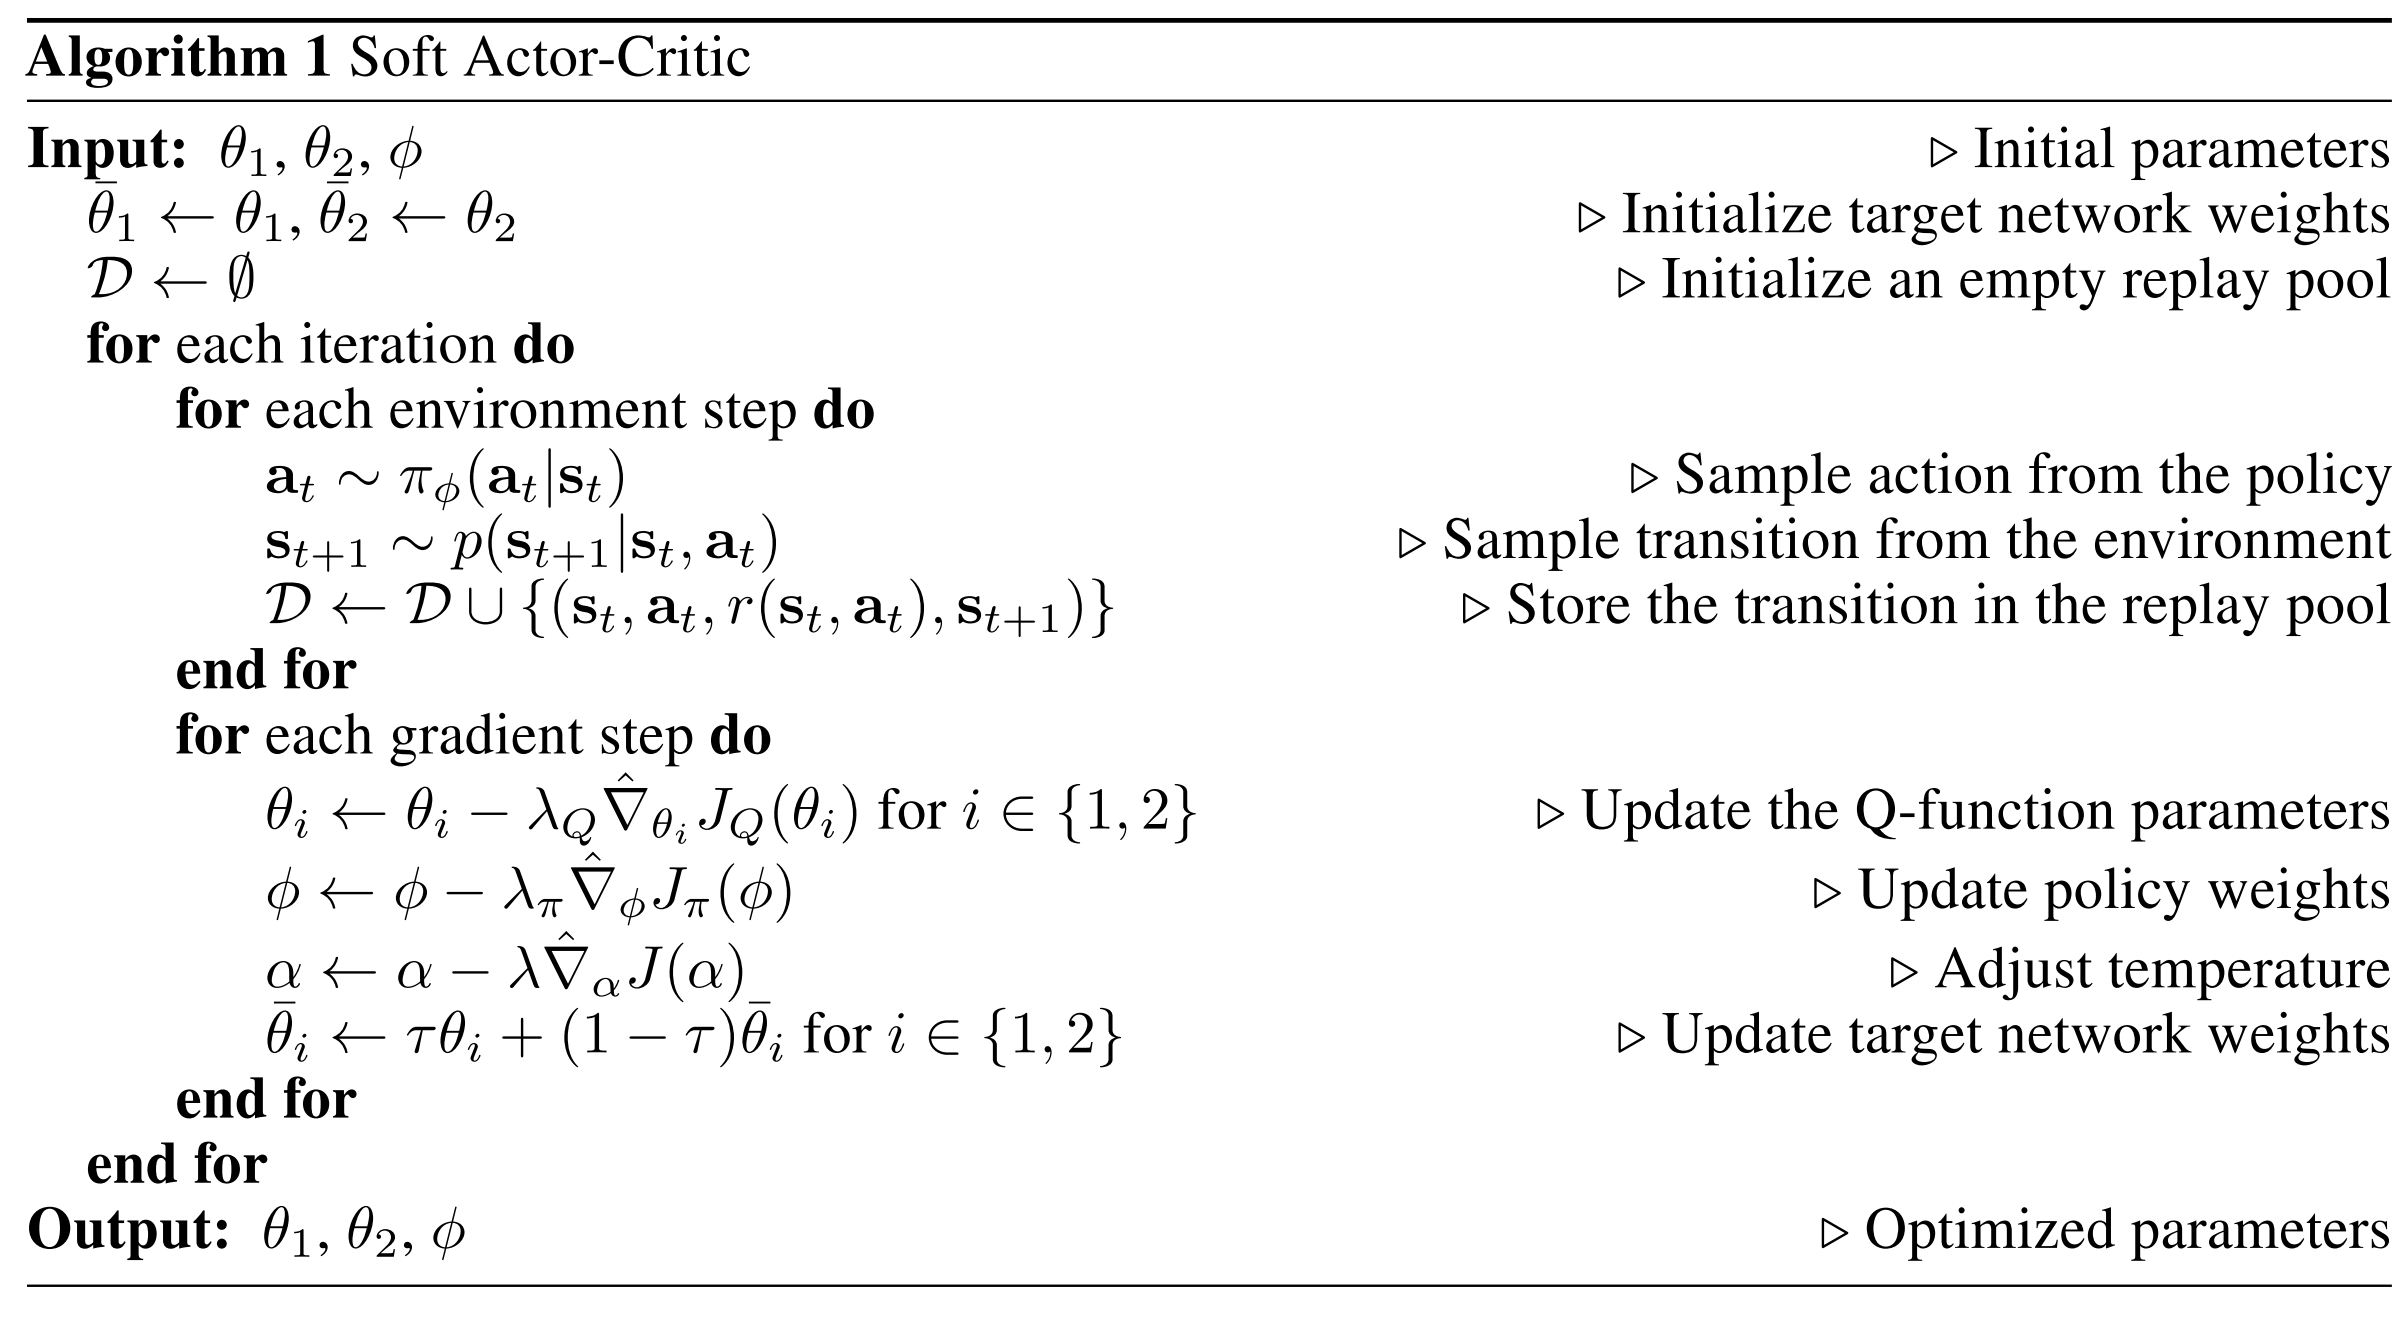
\includegraphics[width=1.0\textwidth]{figures/SACalgo}
    \caption{SAC pseudocode \cite{Haarnoja2018}}
    \label{fig:sacalgo}
\end{figure}
